\chapter{Entropy and Its Interpretations}

Consider a random variable \( X \) taking values in an alphabet \( \mathcal{X} = \{x_1, \dots, x_l\} \).

\defb{Definition: Information Content}{
    The \textit{information content} (also known as surprise or surprisal) of a realisation \( x \) is defined as:
    \[
        h(x) := \log \frac{1}{p(x)}
    \]
}

\defb{Definition: Entropy}{
    The \textit{entropy} of a random variable \( X \) is given by:
    \[
        H(X) := \sum_{x \in \mathcal{X}} p(x) \log \frac{1}{p(x)}
    \]
    Entropy represents the expected value of the information content (or surprisal) across all possible realisations of \( X \):
    \[
        H(X) = \mathbb{E}[h(X)] = \sum_x p(x) h(x)
    \]
}

\section{Entropy of a Biased Coin} \label{sec:entropy_coin}

Let $X$ be a coin flip from a biased coin with alphabet $\mathcal{X} = \{H, T\}$ and probabilities $(p, 1-p)$. The entropy of $X$ is given by the binary entropy function:

\marginnote[-10pt]{This is the expected value of surprisal when flipping a biased coin. }

\[
    H(p) = -p \log p - (1-p) \log (1-p)
\]

\begin{figure*}[h]
    \centering
    \begin{minipage}{0.3\textwidth}
        \centering
        % Plot h(p) = log2(1/p)
        \begin{tikzpicture}
            \begin{axis}[
                    domain=0.001:1,
                    samples=100,
                    width=\textwidth,
                    height=0.8\textwidth,
                    xlabel={$p$},
                    ylabel={$h(p)$},
                    ytick={0,2,4,6,8,10},
                    ymin=0, ymax=10,
                    xmin=0, xmax=1,
                    axis lines=left,
                    every axis y label/.style={at={(current axis.above origin)},anchor=south},
                    every axis x label/.style={at={(current axis.right of origin)},anchor=west}
                ]
                \addplot[black, thick] {log2(1/x)};
                \node[above right] at (axis cs:0.3,7) {$h(p) = \log_2 \frac{1}{p}$};
            \end{axis}
        \end{tikzpicture}
    \end{minipage}
    \hfill
    \begin{minipage}{0.3\textwidth}
        \centering
        % Table for values of p, h(p), and H2(p)
        \renewcommand{\arraystretch}{1.2}
        \begin{tabular}{ccc}
            \hline
            $p$   & $h(p)$ & $H_2(p)$ \\
            \hline
            0.001 & 10.0   & 0.011    \\
            0.01  & 6.6    & 0.081    \\
            0.1   & 3.3    & 0.47     \\
            0.2   & 2.3    & 0.72     \\
            0.5   & 1.0    & 1.0      \\
            \hline
        \end{tabular}
    \end{minipage}
    \hfill
    \begin{minipage}{0.3\textwidth}
        \centering
        % Plot H2(p) = -p*log2(p) - (1-p)*log2(1-p)
        \begin{tikzpicture}
            \begin{axis}[
                    domain=0.001:1,
                    samples=100,
                    width=\textwidth,
                    height=0.8\textwidth,
                    xlabel={$p$},
                    ylabel={$H_2(p)$},
                    ymin=0, ymax=1,
                    xmin=0, xmax=1,
                    axis lines=left,
                    every axis y label/.style={at={(current axis.above origin)},anchor=south},
                    every axis x label/.style={at={(current axis.right of origin)},anchor=west}
                ]
                \addplot[black, thick] {-x*log2(x) - (1-x)*log2(1-x)};
                \node[above] at (axis cs:0.5,0.5) {$H_2(p)$};
            \end{axis}
        \end{tikzpicture}
    \end{minipage}
    \vspace{10pt}
    \caption{Unlikely outcomes provide more information – but if the outcomes of the coin are skewed towards one side, the overall entropy decreases, because the extra information gained by the rarer outcome is diminished by the expectation, where it doesn't happen often enough, reducing the total expected surprise.}
    \label{fig:entropy_coin}
\end{figure*}

Mathematically, a biased coin flip $X$ is just the \textbf{Bernoulli distribution} with parameter $p$:
\[
    X \sim \mc{B}(p)
\]

\sn{The units of \ensuremath{h(x)}}{
    The units of $h(x)$ depend on the base of the log– $\log_2$ is for bits, $\log_{10}$ is for dits, and $\log_e$ is for nats.
}

\defb{Terminology of `Bit'}{
    We denote two things with \textbf{bit}:
    \begin{enumerate}
        \item The units of information content, taken with $\log_2$.
        \item A random variable with alphabet $\{0, 1\}$.
    \end{enumerate}
}

\section{Properties of Entropy in Discrete Distributions}

\begin{itemize}
    \item The entropy of discrete distributions is non-negative.
    \item The general bound on discrete entropy is \( 0 \leq H(X) \leq \log |\mathcal{X}| \).
    \item Entropy is minimised for the Kronecker delta distribution, (i.e. $p_i = 1, p_{j \neq i} = 0$). For example, take the Kronecker delta function \(\delta_{i3}\):
          \[
              \delta_{i3} = \begin{cases}
                  1 & \text{if } i = 3 \\
                  0 & \text{otherwise}
              \end{cases}
          \]
          \begin{center}
              \begin{tikzpicture}
                  % Set up the axis
                  \draw[->] (-0.5,0) -- (6.5,0) node[right] {$i$};  % x-axis
                  \draw[->] (0,-0) -- (0,1.5) node[above] {$\delta_{i3}$}; % y-axis

                  % Label x-axis values
                  \foreach \x in {0, 1, 2, 3, 4, 5, 6}
                  \draw (\x,0) -- (\x,-0.1) node[below] {\x};

                  % Draw Kronecker delta "spikes"
                  \foreach \x in {0, 1, 2, 4, 5, 6}
                  \draw[thick] (\x, 0) -- (\x, 0); % Zero-height "bars"

                  % Draw the "spike" at i = 3
                  \filldraw[blue] (3,0) rectangle (3.04,1);  % Bar at i = 3
                  \node[above, blue] at (3,1) {1};  % Label the height of the delta function

                  % Label for Kronecker delta
                  \node[right] at (3.2, 1) {\(\delta_{i3}\)};
              \end{tikzpicture}
          \end{center}
          Calculating entropy for this distribution:
          \[
              H(X) = \left( 1 \cdot \log 1 + \sum_{i \neq 3} 0 \cdot \log 0 \right) = 0
          \]

    \item Entropy is maximised for the uniform distribution
\end{itemize}

\intuitb{Impossible Events– What if \ensuremath{p_j = 0}?}{
    The mathematical convention is to treat $0 \log 0 = 0$ – impossible events do not change entropy.
}


\section{Independent Random Variables}

What happens if I flip two coins separately? Consider two independent flips $X$ and $Y$. Recall for independent RVs, $P(X, Y) = P(X)P(Y)$. The joint entropy of $X$ and $Y$ is given by:

\begin{align*}
    h(x, y) & = -\log P(x, y)             \\
            & = -\log \big(P(x) P(y)\big) \\
            & = -\log P(x) - \log P(y)    \\
            & = h(x) + h(y)
\end{align*}

Similarly for entropy, note that \textbf{entropy is additive for independent random variables:}


\begin{align*}
    H(X, Y) & = \sum_{\textcolor{blue}{x}, \textcolor{red}{y}} P(x, y) h(x, y)                                                                                                      \\
            & = \sum_{\textcolor{blue}{x}, \textcolor{red}{y}} \textcolor{blue}{P(x)} \textcolor{red}{P(y)} h(x, y) + \sum_{\textcolor{blue}{x}, \textcolor{red}{y}} P(x) P(y) h(y) \\
            & = \textcolor{red}{\cancel{\underbrace{\sum_{y} \textcolor{red}{P(y)}}_{\textcolor{red}{1}}}}
    \cdot \textcolor{blue}{\sum_{x} \textcolor{blue}{P(x)} h(x)}
    + \cancel{\underbrace{\sum_{x} P(x)}_{1}} \cdot \sum_{y} P(y) h(y)                                                                                                              \\
            & = \textcolor{blue}{H(X)} + H(Y).
\end{align*}

\defb{Shannon Axioms}{
    The surprisal of an event with probability \( p \), \( i(p) \) must satisfy:
    \begin{enumerate}
        \item Certain events are unsurprising: \( i(1) = 0 \).
        \item Less probable events are more surprising: \( \frac{di}{dp} \leq 0 \).
        \item Independent events yield the sum of their surprisals:
              \[
                  i(p \cdot q) = i(p) + i(q).
              \]
    \end{enumerate}
    The only function satisfying these axioms is the negative logarithm:
    \[
        i(p) = h(p) = -\log_b(p)
    \]

    \textit{Note: There are many equivalent sets of axioms for entropy.}
}

\section{Information Gain}

\subsection{A Number Guessing Game}

In the game \textit{Who's Who}, one player picks a character, and the other asks yes-or-no questions to guess their identity, such as:
\begin{itemize}
    \item Are they wearing glasses?
    \item Do they have a moustache?
\end{itemize}

To explore a simpler variation, consider a game called \textit{Sixty-Three}:
\begin{itemize}
    \item One player selects an integer \( x \) from 0 to 63.
    \item The other player asks questions to guess \( x \).
\end{itemize}

\textbf{Optimal Questions:} One possible set of optimal questions:
\begin{enumerate}
    \item Is \( x \geq 32 \)?
    \item Is \( x \mod 32 \geq 16 \)?
    \item \dots
    \item Is \( x \mod 2 = 1 \)?
\end{enumerate}

This strategy defines a map \( \{0, \dots, 63\} \to \{0,1\}^6 \), where each output bit is the answer to a specific question. For example, \( x = 35 \) corresponds to \( 100011 \).

If \( x \) is uniformly distributed, each answer provides 1 bit of information, calculated as \( h = -\log(1/2) = 1 \) bit. Thus, the total information gained is 6 bits.

Information content corresponds to the length of the binary encoding of \( x \).

\subsection{A Submarine Guessing Game}

\begin{itemize}
    \item I pick one of 64 squares to hide a submarine.
    \item In each round, you fire at one square, resulting in a ‘hit’ or ‘miss.’
\end{itemize}

(The difference with \textit{sixty-three} is that you always fire to just one square.)

\begin{figure*}
    \centering
    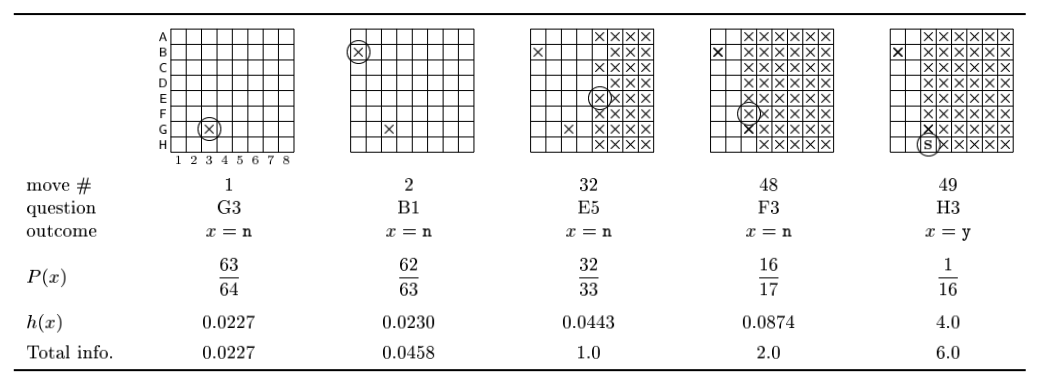
\includegraphics[width=0.9\linewidth]{img/submarines.png}
\end{figure*}

\begin{itemize}
    \item \textbf{Scenario 1:} You hit the submarine with the first question.
          \begin{itemize}
              \item You obtain \( \log(64) = 6 \) bit.
          \end{itemize}

    \item \textbf{Scenario 2:} You miss 32 times, then hit.
          \begin{itemize}
              \item The first miss gives you \( \log(64/63) = 0.0227 \) bit.
              \item By the 32\textsuperscript{nd} miss, you have
                    \[
                        \log(64/63) + \log(63/62) + \dots + \log(33/32) = 0.0227 + 0.0230 + \dots + 0.0444 = 1 \text{ bit}.
                    \]
              \item The hit gives you \( \log(32) = 5 \) bit, for a total of 6 bit.
          \end{itemize}

    \item \textbf{General case:} You miss \( 64 - n \), then hit:
          \[
              \underbrace{\log \frac{64}{63} + \log \frac{63}{62} + \dots + \log \frac{n+1}{n}}_{\text{misses}} + \underbrace{\log \frac{n}{1}}_{\text{hit}} = \log 64 = 6 \text{ bit}
          \]

    \item \textbf{Conclusion:} Regardless of when you hit, you always get 6 bit.
\end{itemize}

\intuitb{Conclusions}{
    \begin{itemize}
        \item For uniform distributions, \( h(x) \) corresponds to the length of the \textbf{binary representation} of \( x \) (i.e., number of yes/no questions).

        \item \( h(x) \) is a measure of the \textbf{“intrinsic”} information content of \( x \), regardless of how that information is obtained.

        \item Information is given by \textbf{probability mass exclusions} (Hartley 1928).
    \end{itemize}

    The goal of experiments is to \textbf{reduce uncertainty} about something by excluding possibilities. The takeaway is that you should design experiemtns with evenly probable outcomes to maximise information gain, as shown in Figure \ref{fig:entropy_coin}.
}

\section{Entropy in Continuous Distributions}

We have explored entropy in discrete RVs with finite alphabets, we then extend this to continuous RVs– by discretising the variable's continous domain.

\begin{itemize}
    \item We have a random variable \( X \in \mathbb{R} \) with PDF \( f(x) \).
    \item We use bins of width \( \Delta \) to get a discrete variable \( X^{\Delta} \) with
          \[
              p_i = \int_{(i - \frac{1}{2})\Delta}^{(i + \frac{1}{2})\Delta} f(x) \, dx = f(x_i) \Delta
          \]
    \item Now we take \( H(X^{\Delta}) \) as \( \Delta \to 0 \):
          \begin{align*}
              H(X^{\Delta}) & = -\sum p_i \log p_i                                                                                                         \\
                            & = -\sum f(x_i) \Delta \log(f(x_i) \Delta)                                                                                    \\
                            & = -\sum \Delta f(x_i) \log f(x_i) - \log \Delta                                                                              \\
                            & = \underbrace{-\sum \Delta f(x_i) \log f(x_i)}_{\text{Riemann integral}}  \underbrace{- \log \Delta}_{\text{Divergent term}}
          \end{align*}
    \item Oh no, \( \lim_{\Delta \to 0} \log \Delta = -\infty \), so \( H(X^{\Delta}) \) diverges for any \( f(x) \).
    \item A foolproof strategy is to ignore $\log \Delta$ anyway, and define the \textbf{differential entropy} as:
\end{itemize}

\defb{Definition: Differential entropy}{
    The \textit{differential entropy} of a continuous RV \( X \) with PDF \( f(x) \) is given by
    \[
        H(X) := - \int f(x) \log f(x) \, dx
    \]
}

\sn{Warning}{
    The \( \log \Delta \) will come back to haunt us! Differential entropy lacks many interesting properties of discrete entropy. \bigskip

    \textbf{Disclaimer:} We may use the term ‘entropy’ for continuous RVs too.
}

\subsection{Properties of Differential Entropy}
Take an example of differential entropy in uniform distributions:
Let \( X \) be a uniform random variable in the interval of length \( a \).

\[
    X \sim \mathcal{U}([0, a]) \quad \text{i.e.} \quad p(x) = \frac{1}{a}
\]

\[
    H(X) = - \int_0^a \frac{1}{a} \log \frac{1}{a} \, dx = - \log \frac{1}{a} \int_0^a \frac{dx}{a} = \log a
\]

\textbf{Conclusions:} We see that Differential entropy:
\begin{itemize}
    \item Can be negative, e.g. for $a < 1$.
    \item Grows with the volume of the distribution $(2^{H(X)} = a > 0)$
\end{itemize}

\subsection{Surprisal in Gaussian Distributions}

\marginnote{\intuitsb{Modelling \ensuremath{x}}{We want to reduce surprisal to ensure we can compactly encode $x$ more efficiently. In this example, we want to model \( x \) with the Gaussian distribution. Reducing surprisal is then equivalent to reducing the prediction error, or the mean squared error (MSE). \bigskip

        Try to imagine a distribution of $x$ and then we play around with the parameters of a Gaussian distribution to make it fit the distribution of $x$ better. \bigskip

        If we find a more accurate $\mu$ for our model, we then reduce the MSE. And if our $\mu$ is already quite close to the true value of $x$, increasing precision (making reducing $\sigma$ to make the distribution more narrow, centring closer around $\mu$) can also sometimes reduce surprisal. However, if $\mu$ is too far from the true value of $x$, increasing precision can sometimes increase surprisal.}}

Let \( X \sim \mathcal{N}(\mu, \sigma^2) \) be a 1D Gaussian random variable, i.e.
\[
    p(x) = \left( \sigma \sqrt{2 \pi} \right)^{-1} e^{-\frac{1}{2} \left( \frac{x - \mu}{\sigma} \right)^2}
\]


Then, surprisal is just the negative $ln$ of the PDF:
\[
    h(x) = \ln \left( \sigma \sqrt{2 \pi} \right) + \frac{1}{2} \left( \frac{x - \mu}{\sigma} \right)^2
\]

This expression is equivalent to scaled mean squared error (MSE):
\[
    h(x) = \ln \sigma + \frac{1}{2 \sigma^2} \text{MSE}(x, \mu) + C.
\]

If we predict \( x \) with a PDF \( \mathcal{N}(\mu, \sigma^2) \), we can lower the surprisal by:

\begin{itemize}
    \item Reducing the bias (i.e., moving \( \mu \) closer to \( x \)),
    \item (Sometimes) increasing the precision (i.e., increasing \( \sigma \)).
\end{itemize}


\subsection{Entropy in Gaussian Distributions}

We show that Entropy has a closed-form expression for Gaussian Distributions:

To calculate the entropy of a \(D\)-dimensional Gaussian distribution \(\mathcal{N}(\mu, \Sigma)\),

\[
    p(x) = |2 \pi \Sigma|^{-1/2} \exp \left( -\frac{1}{2} (x - \mu)^\top \Sigma^{-1} (x - \mu) \right).
\]

The entropy \(H(X)\) is given by:
\[
    H(X) = - \int_{-\infty}^{+\infty} \mathcal{N}(x; \mu, \Sigma) \ln \mathcal{N}(x; \mu, \Sigma) \, dx.
\]

Expanding, we get:
\[
    H(X) = \frac{1}{2} \mathbb{E}[\ln |2 \pi \Sigma|] + \frac{1}{2} \mathbb{E}[(x - \mu)^\top \Sigma^{-1} (x - \mu)].
\]

For the first term, \(\mathbb{E}[\ln |2 \pi \Sigma|] = \ln |2 \pi \Sigma|\).

For the second term:
\[
    \mathbb{E} \left[ (x - \mu)^\top \Sigma^{-1} (x - \mu) \right] = \operatorname{tr} \left( \Sigma^{-1} \mathbb{E} \left[ (x - \mu)(x - \mu)^\top \right] \right) = \operatorname{tr}(\Sigma^{-1} \Sigma) = D.
\]

Substituting back, we get:
\begin{align*}
    H(X) & = \frac{1}{2} \ln |2 \pi \Sigma| + \frac{1}{2} D = \frac{1}{2} \ln \left( |2 \pi \Sigma| e^D \right) \\ &= \frac{1}{2} \ln |2 \pi e \Sigma|.
\end{align*}



\defb{Entropy of a Gaussian}{
    For a \(D\)-dimensional Gaussian distribution \(\mathcal{N}(\mu, \Sigma)\), the entropy is given by:
    \[
        H(X) = \frac{1}{2} \ln |2 \pi e \Sigma|.
    \]
}\label{def:gaussian_entropy}

\subsection{Takeaways of Entropy}
\begin{itemize}
    \item Entropy quantifies the \textbf{average information content} of an observation \(x\).
    \item Entropy serves as a \textbf{generalised variance} (e.g., measures predictability of \(X\)).
    \item For discrete distributions:
          \begin{itemize}
              \item Entropy is \textbf{bounded}: \(0 \leq H(X) \leq \log |\mathcal{X}|\).
              \item Related to the \textbf{number of yes/no questions} needed to determine \(x\).
          \end{itemize}
    \item For continuous distributions, \textbf{differential entropy} is defined, but can be negative and lacks some properties of discrete entropy.
\end{itemize}

\section{Prerequisites before the Source Coding Theorem}

\defb{Definition: Code and Code Length}{
    Given a random variable \( X \) with alphabet \( \mathcal{X} \) and an alphabet \( \mathcal{D} \), a \textbf{code} is a mapping
    \[
        C : \mathcal{X} \to \mathcal{D}^*,
    \]
    where \( \mathcal{D}^* \) is the set of all finite-length strings of symbols in \( \mathcal{D} \).

    The quantity \( \ell(x) \) is the \textbf{code length} of \( C(x) \), and \( L = \mathbb{E}[\ell(x)] \) the \textbf{average code length}.
}

\begin{itemize}
    \item For each symbol \( x \), the string \( C(x) \in \mathcal{D}^* \) is called a \textbf{codeword}.
    \item When \( |\mathcal{D}| = 2 \), \( C \) is a \textbf{binary code}. When \( |\mathcal{D}| = d \), \( C \) is a \textbf{d-ary code}.
\end{itemize}

Here are two example codes for the alphabet \( \mathcal{X} = \{ \text{a}, \text{b}, \text{c}, \text{d} \} \).

\begin{table}[h]
    \centering
    \begin{tabular}{c@{\hskip 1cm}c}
        \begin{tabular}{cc}
            \toprule
            \multicolumn{2}{c}{Binary} \\
            \midrule
            \( x \) & \( C(x) \)       \\
            \midrule
            a       & 00               \\
            b       & 01               \\
            c       & 10               \\
            d       & 11               \\
            \bottomrule
        \end{tabular}
         &
        \begin{tabular}{cc}
            \toprule
            \multicolumn{2}{c}{Ternary} \\
            \midrule
            \( x \) & \( C(x) \)        \\
            \midrule
            a       & 0                 \\
            b       & 1                 \\
            c       & 2                 \\
            d       & 200               \\
            \bottomrule
        \end{tabular}
    \end{tabular}
\end{table}


\subsection{Coding for the Uniform Distribution}

\begin{itemize}
    \item We’ve seen that (in uniform distributions), entropy corresponds to the number of \textbf{yes/no} questions needed to guess \( x \).

          \[
              \begin{array}{c@{\quad\Rightarrow\quad}c@{\quad}c@{\quad\Rightarrow\quad}c}
                  35 & 100011 & 6     & 000110 \\
                  0  & 000000 & 17    & 010001 \\
                  42 & 101010 & \dots & \dots  \\
              \end{array}
          \]

    \item This forms a \textbf{binary code} for \( X \) with length
          \[
              L = H(X) = \log |\mathcal{X}|.
          \]

    \item More generally, \( \log |\mathcal{X}| \) is referred to as the \textbf{raw bit content} of \( X \).
\end{itemize}

\sn{Warning: Ceiling and the “Extra Bit”}{
    When \( |\mathcal{X}| \) is not a power of two, we may need an “extra bit” to encode symbols. You may see this written as \( L = \lceil \log |\mathcal{X}| \rceil \) or \( L = \log |\mathcal{X}| + 1 \).
}


\subsection{Non-uniform Distributions}

What happens when the distribution isn’t uniform?



\begin{itemize}
    \item \textbf{Example}: compressing Wikipedia, which has alphabet \( \mathcal{X} = \mathcal{E} \cup \mathcal{U} \):
          \begin{itemize}
              \item \( \mathcal{E} \) is the English alphabet, \( |\mathcal{E}| = 26 \);
              \item \( \mathcal{U} = \{ !, @, \#, \$, \%, -, \&, *, (, ) \} \) includes some unicode characters.
          \end{itemize}

    \item Assume that 98\% of Wikipedia content comes from \( \mathcal{E} \), and 2\% from \( \mathcal{U} \).

    \item A naive binary code of \( \mathcal{X} \) would require \( \lceil \log |\mathcal{X}| \rceil = \lceil \log 36 \rceil = 6 \) bits.

    \item \textbf{But}... if we ignore \( \mathcal{U} \), we can encode in \( \lceil \log |\mathcal{E}| \rceil = \lceil \log 26 \rceil = 5 \) bits.
\end{itemize}

\sn{Reduction in Code Length}{
    We have \textbf{reduced the code length} with only \textbf{2\% error}, simply by refusing to encode the minority of rarely-used symbols. And this generally would not have a major impact on the readability of the text– most information could still be conveyed.
}


\section{Law of Large Numbers}

The Law of Large Numbers states that as the number of independent, identically distributed (i.i.d.) random variables increases, their sample average converges to the expected value. This result forms a cornerstone of probability and statistics, establishing that with a large enough sample size, we can expect the sample mean to approximate the population mean closely.

\begin{itemize}
    \item Let \( Y^n = \frac{1}{n} \sum_{i=1}^n X_i \) be the mean of \(n\) i.i.d. random variables \( X_1, \dots, X_n \), with
          \[
              \mathbb{E}[X_1] = \dots = \mathbb{E}[X_n] = \mu \quad \text{and} \quad \operatorname{Var}(X_i) = \dots = \operatorname{Var}(X_n) = \sigma^2.
          \]

    \item By direct calculation, it can be shown that:
          \[
              \mathbb{E}[Y^n] = \mu \quad \text{and} \quad \operatorname{Var}(Y^n) = \frac{\sigma^2}{n}.
          \]

    \item As \( n \to \infty \), \( Y^n \) has \textbf{vanishing variance}, meaning \( Y^n \) becomes increasingly close to \( \mu \).
\end{itemize}

\thm{Weak Law of Large Numbers}{
    Let \( Y^n = \frac{1}{n} \sum_{i=1}^n X_i \). As \( n \to \infty \), \( Y^n \) converges in probability to \( \mu \):
    \[
        Y^n \xrightarrow{P} \mu, \quad \text{that is,} \quad \lim_{n \to \infty} \Pr\left( |Y^n - \mu| < \varepsilon \right) = 1
    \]
    for any \( \varepsilon > 0 \).
}

\section{High-Dimensional Spaces}

Life in high-dimensional spaces can be weird, or in a sense, behave geometric properties behave in unintuitive ways. Consider an $n$-dimensional Gaussian random variable:

\[
    X \sim N(0, \sigma^2 I_n),
\]

where each component $X_i$ of $X$ is independent and identically distributed (i.i.d.) as $N(0, \sigma^2)$. This means that each component has zero mean and variance $\sigma^2$.

To explore the geometry of high-dimensional spaces, we examine the squared Euclidean distance from the origin, given by

\[
    r^2 = \| X \|^2 = x_1^2 + x_2^2 + \dots + x_n^2 = \sum_{i=1}^n x_i^2.
\]

Applying the Law of Large Numbers (LLN), we see that as $n$ becomes large, the distribution of the distances from the origin concentrates around its expected value. Thus, most points are found approximately at the same distance from the origin, rather than spread out.

\subsection{Concentration of Measure}

As we compute the expected squared distance from the origin, we find

\[
    \mathbb{E}[r^2] = n \, \mathbb{E}[X_i^2] = n \sigma^2,
\]

and the variance of this squared distance is given by

\[
    \text{Var}(r^2) = n \, \text{Var}(X_i^2).
\]

The standard deviation relative to the mean distance decreases as $n$ grows, as shown by

\[
    \frac{\text{Std}(r^2)}{\mathbb{E}[r^2]} = \frac{\sqrt{\text{Var}(r^2)}}{\mathbb{E}[r^2]} = \mathcal{O}\left(\frac{1}{\sqrt{n}}\right) \quad \text{as} \quad n \to \infty.
\]

This implies that in high-dimensional spaces, random points are highly likely to lie within a thin spherical shell at a nearly fixed distance from the origin, with the thickness of the shell shrinking relative to its radius as $n$ increases. \footnote{This phenomenon is known as concentration of measure.}

\begin{figure}
    \centering
    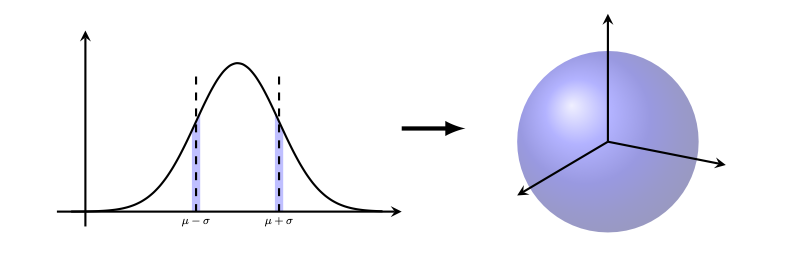
\includegraphics[width=\linewidth]{img/life_hd_space.png}
    \caption{Most, if not all points live in a shell at the same distance from the origin.}
\end{figure}

The consequences of this are profound for high-dimensions, as intuitions based on low-dimensional space often fail. For instance, in high dimensions, most of the ``volume" of a space is near the surface, not in the core, which affects probability distributions, sampling methods, and the geometry of high-dimensional objects. This brings us to the Asymptotic Equipartition Property (AEP).


\section{Asymptotic Equipartition Property (AEP)}

\thm{Theorem: AEP}{
    Let $X_1, \dots, X_n$ be i.i.d. random variables drawn from a distribution with probability mass function $p(x)$. Then, as $n \to \infty$:
    \[
        \lim_{n \to \infty} -\frac{1}{n} \log p(X_1, \dots, X_n) = H(X),
    \]
    where $H(X)$ is the entropy of $X$.

    \paragraph{Proof: }
    \begin{enumerate}
        \item Rewrite the log-probability of a sequence as a sum:
              \[
                  -\frac{1}{n} \log p(X_1, \dots, X_n) = -\frac{1}{n} \sum_{i=1}^n \log p(X_i).
              \]
        \item By the Weak Law of Large Numbers, the average $\frac{1}{n} \sum_{i=1}^n -\log p(X_i)$ converges to its expected value, $H(X)$, as $n$ grows.
        \item Thus, for large $n$, $-\frac{1}{n} \log p(X_1, \dots, X_n)$ is close to $H(X)$.
    \end{enumerate}
}

\textbf{Interpretation}: The AEP states that for a large number of i.i.d. samples, almost all observed sequences will have approximately the same probability, $2^{-nH(X)}$. This means that the probability of a specific sequence from the typical set becomes nearly uniform. This foundational because it implies that in the limit, most sequences are effectively indistinguishable in probability.

\section{Properties of the Typical Set}
\marginnote[5.5pt]{
    \ex{More coin flips}{
        A group of \(n\) people flip a biased coin (\(p = 0.2\)) at the same time, and write down the number of heads. As \(n\) grows, almost all the time we will get very close to \(20\%\) of coins being heads.

        \begin{center}
            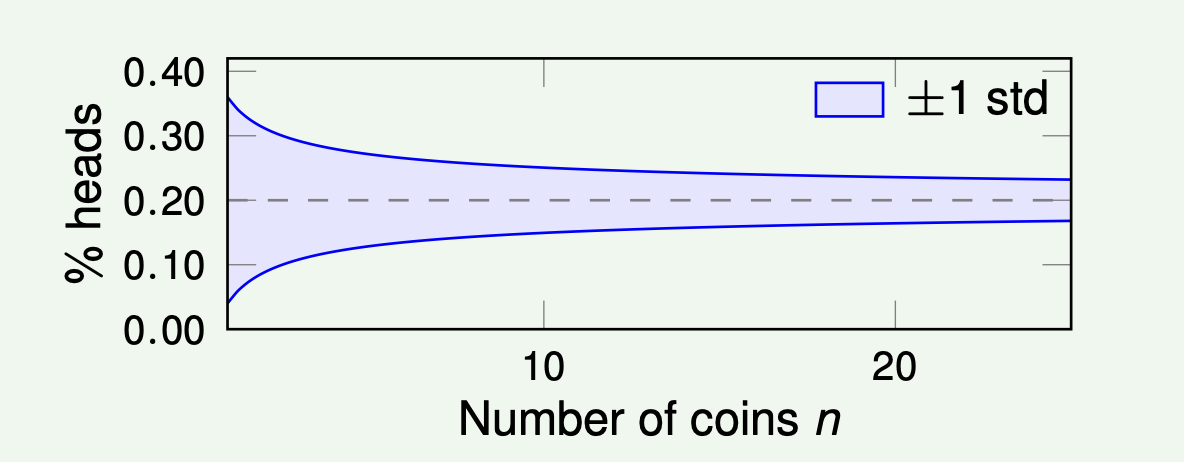
\includegraphics[width=\linewidth]{img/biased_coin_aep}
        \end{center}
    }
}

\defb{Typical Set}{
    \raggedright
    The \textbf{typical set} $A^{(n)}_\epsilon$ for a small $\epsilon > 0$ is defined as the set of sequences $x_1, \dots, x_n$ that satisfy:
    \[
        2^{-n(H(X) + \epsilon)} \leq p(x_1, \dots, x_n) \leq 2^{-n(H(X) - \epsilon)}.
    \]
    This set captures the outcomes that are most likely to occur when sampling $n$ times from the distribution of $X$.

}
The typical set has the following important properties:
\begin{enumerate}
    \item \textbf{Uniformity of Probabilities:} For any sequence $x^n \in A^{(n)}_\epsilon$, we have:
          \[
              H(X) - \epsilon \leq -\frac{1}{n} \log p(x^n) \leq H(X) + \epsilon.
          \]
          This implies that all samples (or sequences) in the typical set $A_\epsilon^{(n)}$ have approximately equal probabilities (uniformly distributed), so $p(x^n) \approx 2^{-nH(X)}$, regardless of the specific sequence $x^n$.

          \textbf{Proof:} This follows directly from the definition of $A^{(n)}_\epsilon$. By construction, all sequences in the typical set satisfy $-\frac{1}{n} \log p(x^n)$ close to the entropy $H(X)$, with only a small deviation $\epsilon$.

    \item \textbf{High Probability of Occurrence:} The probability that a randomly chosen sequence falls within the typical set is very high:
          \[
              P(x^n \in A^{(n)}_\epsilon) > 1 - \epsilon.
          \]
          Therefore, as $n$ becomes large, almost all observed sequences will belong to the typical set.

          \textbf{Proof:}
          \begin{itemize}
              \item For $x_1, \dots, x_n$ drawn from $X$, the average log-probability can be written as:
                    \[
                        -\frac{1}{n} \log p(x_1, \dots, x_n) = -\frac{1}{n} \sum_{i=1}^n \log p(x_i).
                    \]
              \item By the Weak Law of Large Numbers, as $n \to \infty$, this average converges to its expected value $H(X)$, with a variance that tends to zero.
              \item This implies that the probability of the sample average deviating from $H(X)$ by more than $\epsilon$ becomes negligible as $n$ grows, ensuring that $P(x^n \in A^{(n)}_\epsilon) \to 1$ as $n \to \infty$.
          \end{itemize}

    \item \textbf{Upper Bound on Set Size:} The number of sequences in the typical set is bounded above by:
          \[
              |A^{(n)}_\epsilon| \leq 2^{n(H(X) + \epsilon)}.
          \]
          This implies that the typical set contains at most $2^{n(H(X) + \epsilon)}$ sequences, which is only a small fraction of the $2^n$ possible sequences as $n$ grows.

          \textbf{Proof:}
          \begin{itemize}
              \item Since $p(x^n) \approx 2^{-nH(X)}$ for sequences in the typical set, the sum of probabilities over all sequences in $A^{(n)}_\epsilon$ gives
                    \[
                        \sum_{x^n \in A^{(n)}_\epsilon} p(x^n) \leq |A^{(n)}_\epsilon| \cdot 2^{-n(H(X) - \epsilon)}.
                    \]
              \item Given that the total probability mass is 1, we find
                    \[
                        |A^{(n)}_\epsilon| \cdot 2^{-n(H(X) - \epsilon)} \leq 1 \Rightarrow |A^{(n)}_\epsilon| \leq 2^{n(H(X) + \epsilon)}.
                    \]
          \end{itemize}

    \item \textbf{Lower Bound on Set Size:} The size of the typical set is also bounded below by:
          \[
              |A^{(n)}_\epsilon| \geq (1 - \epsilon) 2^{n(H(X) - \epsilon)}.
          \]
          This ensures that the typical set captures nearly all the probability mass, containing close to $2^{nH(X)}$ sequences.

          \textbf{Proof:}
          \begin{itemize}
              \item Since $P(x^n \in A^{(n)}_\epsilon) > 1 - \epsilon$, we have
                    \[
                        \sum_{x^n \in A^{(n)}_\epsilon} p(x^n) > 1 - \epsilon.
                    \]
              \item For each sequence in the typical set, $p(x^n) \approx 2^{-n(H(X) + \epsilon)}$, so
                    \[
                        (1 - \epsilon) \leq |A^{(n)}_\epsilon| \cdot 2^{-n(H(X) + \epsilon)}.
                    \]
              \item Rearranging gives the lower bound:
                    \[
                        |A^{(n)}_\epsilon| \geq (1 - \epsilon) 2^{n(H(X) - \epsilon)}.
                    \]
          \end{itemize}
\end{enumerate}




\subsection{Typical Set: Intuitions}

The Asymptotic Equipartition Property (AEP) divides the set of all possible events into two categories:

\begin{itemize}
    \item \textbf{Typical Set}: Consists of events that occur almost always when sampling large sequences of random variables. These events are approximately uniform in distribution, with each having nearly the same probability.
    \item \textbf{Non-Typical Set}: Contains the remaining events, which are much less likely to occur.
\end{itemize}


\ex{Typical Set of Biased Coins}{

    Consider a sequence of \(n\) flips of a biased coin with probability \(p = 0.1\) of landing heads. Let \(r(x^n)\) denote the number of 1’s (heads) in the sequence \(x^n\). The variable \(r\) follows a binomial distribution:

    \[
        p(r) = \binom{n}{r} p^r (1 - p)^{n - r}
    \]

    Two main forces shape the distribution of strings in this setup:
    \begin{itemize}
        \item \textbf{Probability Term, \(p^r (1 - p)^{n - r}\)}: This term suggests that the most likely strings will contain fewer heads (1’s).
        \item \textbf{Combinatorial Term, \(\binom{n}{r}\)}: There are more possible sequences with approximately \( \frac{n}{2} \) heads, which maximises the number of configurations for a given count of heads.
    \end{itemize}

    According to the AEP, these two forces meet \textbf{exactly at} \( r = p \cdot n \), meaning that typical sequences will have nearly exactly \(10\%\) heads. Sequences with significantly fewer or more than \(10\%\) heads are rare and contribute only minimally to the total probability.

}

\subsection{Graphical Representation of the Typical Set}

The diagram below illustrates the division of all possible events into the \textbf{Typical Set} and \textbf{Non-Typical Set} as predicted by the AEP.

\begin{center}
    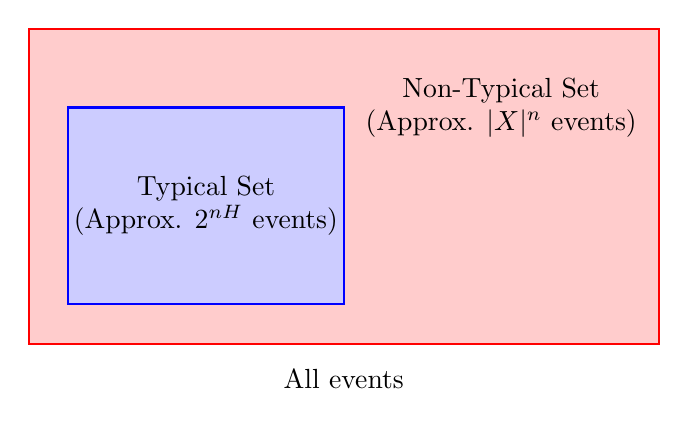
\begin{tikzpicture}
        % Define styles for the circles
        \tikzstyle{typical}=[fill=blue!20, draw=blue, thick]
        \tikzstyle{nontypical}=[fill=red!20, draw=red, thick]

        % Draw the larger rectangle (non-typical set)
        \draw[nontypical, align=center] (0, 0) rectangle (8, 4) node[pos=0.75] {Non-Typical Set\\(Approx. $|X|^n$ events)};

        % Draw the smaller rectangle for the typical set within the non-typical set
        \draw[typical, align=center] (0.5, 0.5) rectangle (4, 3) node[pos=0.5] {Typical Set\\(Approx. $2^{nH}$ events)};

        % Labels
        \node[below] at (4, -0.2) {All events};
    \end{tikzpicture}
\end{center}

This visual helps reinforce the AEP’s implication: almost all of the probability mass for a large sample size is concentrated within the typical set, simplifying coding and probability estimation tasks.


\subsubsection{Entropy and Volume}

The Asymptotic Equipartition Property (AEP) provides a statistical interpretation of entropy as the proportion of the total "volume" occupied by typical outcomes of a random variable \( X \). \bigskip


For binary random variables (where \(|X| = 2\)), the entropy \( H(X) \) represents the fraction of possible events that are likely to occur:

\[
    \frac{\log(\text{\# events that almost always happen})}{\log(\text{\# events that could happen})} = \frac{\log |A^{(n)}_\epsilon|}{\log |X|^n} = \frac{n H(X)}{n} = H(X)
\]

In the case of Gaussian distributions, entropy is proportional (up to an additive constant) to the logarithm of the volume of the isoprobability contours. This volume interpretation highlights the way entropy scales with the ``spread" of the probability distribution:

\begin{figure}[h!]
    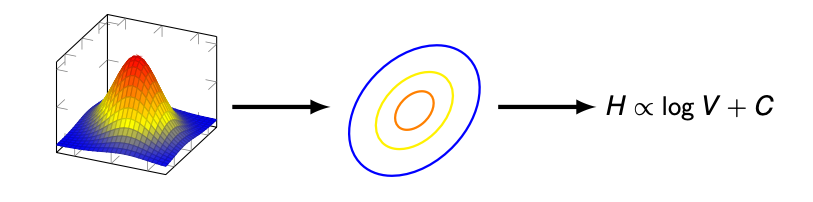
\includegraphics[width=1\linewidth]{img/gaussian_entropy.png}
\end{figure}


\[
    H \propto \log V + C
\]

\subsection{Source Coding Theorem}

\thm{Source Coding Theorem}{
    Let \( X^n \) be an i.i.d. sequence from a probability distribution \( p(x) \). For any \( \epsilon > 0 \), and for sufficiently large \( n \), there exists an invertible code with average length per symbol:
    \[
        E\left[\frac{1}{n} \ell(X^n)\right] \leq H(X) + \epsilon
    \]

    Conversely, it is impossible to construct an invertible code with a shorter average length than \( H(X) \) per symbol.

    \begin{itemize}
        \item This result is a ``limit at infinity" statement following the \((\epsilon, \delta)\) definition.
        \item More precisely: For any \( \epsilon > 0 \), there exists a constant \( N_0 \) such that for all \( n \geq N_0 \), the above inequality holds.
    \end{itemize}

    The theorem consists of two parts:
    \begin{enumerate}
        \item \textbf{Achievability:} There exists a code with average length at most \( H(X) + \epsilon \).
        \item \textbf{Converse (Impossibility):} No code can achieve an average length less than \( H(X) \).
    \end{enumerate}


}




\subsection{Proof of Achievability}

To prove the achievability of the Source Coding Theorem, we construct a specific encoding scheme as follows:

\begin{itemize}
    \item If \( x^n \in A^{(n)}_\epsilon \) (i.e., \( x^n \) belongs to the typical set), we set the first bit to \(0\) and encode the remainder as the binary representation of \( x^n \) within \( A^{(n)}_\epsilon \).
    \item If \( x^n \notin A^{(n)}_\epsilon \) (i.e., \( x^n \) does not belong to the typical set), we set the first bit to \(1\) and encode the remainder as the binary representation of \( x^n \) within \( X^n \).
\end{itemize}

Thus, we can determine the code length \( \ell(x^n) \) as follows:
\begin{itemize}
    \item If \( x^n \in A^{(n)}_\epsilon \), then
          \[
              \ell(x^n) = 1 + \lceil \log |A^{(n)}_\epsilon| \rceil \leq n(H + \epsilon) + 2.
          \]
    \item If \( x^n \notin A^{(n)}_\epsilon \), then
          \[
              \ell(x^n) = 1 + \lceil \log |X|^n \rceil \leq n \log |X| + 2.
          \]
\end{itemize}

\subsubsection{Average Code Length}

The average code length \( L \) can be calculated as:
\[
    L = \sum_{x^n} p(x^n) \ell(x^n).
\]

This expands to:
\begin{align*}
    L & = \sum_{x^n \in A^{(n)}_\epsilon} p(x^n) \ell(x^n) + \sum_{x^n \notin A^{(n)}_\epsilon} p(x^n) \ell(x^n)                                            \\
      & \leq \sum_{x^n \in A^{(n)}_\epsilon} p(x^n) (n(H + \epsilon) + 2) + \sum_{x^n \notin A^{(n)}_\epsilon} p(x^n) (n \log |X| + 2)                      \\
      & = P\left(x^n \in A^{(n)}_\epsilon\right) (n(H + \epsilon) + 2) + \cancel{\left(1 - P\left(x^n \in A^{(n)}_\epsilon\right)\right)} (n \log |X| + 2).
\end{align*}


Using the fact that by AEP, the probability of an occurence in the typical set  \( P\left(x^n \in A^{(n)}_\epsilon\right) \approx 1 \) for large \( n \), this yields:
\begin{align*}
    L & = n(H + \epsilon) + 2 + \epsilon n \log |X| \\
      & = n(H + \epsilon'),
\end{align*}


where \( \epsilon' = \epsilon + \epsilon \log |X| + \frac{2}{n} \).

This completes the proof of achievability, \textbf{Q.E.D.} (quite easily done!).

\subsection{Proof of the Converse (Sketch)}

To show the converse, we consider a hypothetical “sub-typical” set \( C \subset A^{(n)}_\epsilon \) which is smaller than the typical set \( A^{(n)}_\epsilon \). Assume:
\[
    |C| \approx 2^{n(H - \kappa)}
\]
for some \( \kappa > 0 \), meaning that \( C \) would allow us to encode each symbol in \( H - \kappa \) bits.

Since \( C \subset A^{(n)}_\epsilon \), all \( x^n \in C \) satisfy \( p(x^n) \approx |A^{(n)}_\epsilon|^{-1} \). We can compute the probability of sampling from \( C \) as follows:
\[
    P(x^n \in C) = \sum_{x^n \in C} p(x^n) \approx |C| |A^{(n)}_\epsilon|^{-1} \approx 2^{n(H - \kappa)} 2^{-nH} = 2^{-n \kappa}.
\]

As \( n \to \infty \), \( P(x^n \in C) \to 0 \), which implies that the probability of observing sequences within \( C \) vanishes. Thus, trying to compress each symbol in \( H - \kappa \) bits does not actually achieve any saving in a meaningful sense, concluding the converse proof.






\intuitb{Summary on Entropy}{
    \begin{itemize}
        \item \textbf{Entropy represents the \textcolor{blue}{information content} of a random variable (RV).}

        \item \textbf{It is the minimum number of \textcolor{blue}{yes/no questions} needed to guess $x$.}
              \begin{itemize}
                  \item Exactly for uniform distributions.
                  \item Asymptotically for all distributions.
              \end{itemize}

        \item \textbf{It is a quantification of \textcolor{blue}{generalised variance}.}
              \begin{itemize}
                  \item It quantifies how quickly a probability density function (PDF) \textcolor{blue}{fills the space}.
                  \item In Gaussian distributions, it scales with the average mean squared error (MSE).
              \end{itemize}
    \end{itemize}
}









